\chapter{Implementation}

This chapter discusses implementation specifics and the tools used to build smart contracts and jason \ac{BDI} agents. We discuss the \ac{MAS} and \ac{BCT} implementation specifics, package and library versions utilized, and system configuration. Additionally, the procedures necessary to combine both in order to contribute to this thesis are also presented.

\section{System Configuration}

The application was created and tested on a Linux Ubuntu 22.04.1 LTS system.
Visual Studio and InetlliJ are the \ac{IDE}s used to create the application. jEdit is also used somehow to run agents using Jason while creating \texttt{.asl} and running \texttt{.mas2j} file.
To test the compatibility of web3j with gradle for agents, many versions of Java Standard Edition Development Kit were utilized, however the most commonly used was Java SE Development Kit 18.0.2.1. 

\vspace{.5cm}

Other standards for the development of Smart contracts and agents are detailed in the sections below.

\section{Agent Implementation}

The \ac{BDI} architecture is the most common technique to implementing "intelligent" or "rational" agents. The specification of a set of base beliefs and a set of plans results in the creation of an AgentSpeak(L) agent. AgentSpeak(L) differentiates between two kinds of goals: achievement goals and test goals. However, we use achievement targets for our agents. We employed a variety of techniques while writing our agents and ensuring that they could be utilized with smart contracts. We tested several different interpreters and wrote our agents using those. We pursue the following strategies:

\begin{itemize}
    \item \textbf{Jason interpreter built on Java}
    \item \textbf{\ac{ASTRA}}
    \item \textbf{Jason interpreter built on python}
\end{itemize}

The structure of the agent program is governed by the fact that there will be four agents in the MAS, as shown in Figure \ref{Agents in MAS} in MAS, and they will interact with each other as shown in Figure \ref{Agent Interaction}. Our implementation strategy is as follows:

\begin{itemize}
    \item The supply chain will be initiated by the main agent, who will then engage the retailer agent;
    \item Retailer agent will inspect its inventory and sell products to customers; if a product is not in stock, retailer agent will ask the main agent to contact the wholesaler agent;
    \item The wholesaler agent will check its warehouse and ship the product to the retailer agent; if the product is not available, the wholesaler agent will request that the manufacturer agent be contacted by the main agent;
    \item Upon checking its inventory, the manufacturer agent will ship the product to the wholesaler agent. If the product is not in stock, the manufacturer agent will manufacture the product, does the package and deliver it to the wholesaler.
\end{itemize}

Every implementation uses the same approach to how agents cooperate and communicate, and each implementation is detailed in more detail in the section below.

\begin{figure}[h]
\centering
  \includegraphics[width=10cm]{includes/figures/MAS.png} 
  \caption{Agents in \ac{MAS}}
  \label{Agents in MAS}
\end{figure}

\subsection{Jason interpreter built on Java}

AgentSpeak's expanded dialect has an interpreter named Jason. It implements the operational semantics of that language and offers a platform for creating \ac{MAS} with a variety of characteristics that may be altered by the user. Version 3.1 of Jason, which is the most recent version, was installed. The agents are constructed using figure  \ref{Agent Interaction} as a guide.

\vspace{.5cm}

In addition to being able to interpret the original AgentSpeak, Jason possesses a few other crucial abilities. Inter-agent communication based on speech acts and strong negation are included, allowing for the use of both closed- and open-world assumptions. Additionally, it supports creating environments (which are not normally to be programmed in AgentSpeak; in this case they are programmed in Java). It offers the ability to deploy distributed \ac{MAS} via a network (using \ac{JADE}); the user may also add other distribution infrastructures. Furthermore, it offers an \ac{IDE} in the form of an Eclipse or jEdit plugin; the \ac{IDE} has a "mind inspector" that aids with debugging.

\subsection{\ac{ASTRA} Implementation}

\ac{ASTRA} programs are divided into agent classes, which may be expanded using a multiple inheritance paradigm. Each agent class is written in a separate file with the same name as the agent class and the \texttt{.astra} extension. \ac{ASTRA} is distinct from AgentSpeak (L). Because \ac{ASTRA} applications can refer to Java classes, support for delivering fully qualified class names is required. \ac{ASTRA} programs incorporate partial plans (called plan bodies) in addition to plan rules to promote code/class resuability. \ac{ASTRA} strives to be familiar to developers who are familiar with mainstream programming languages, particularly Java.

 \vspace{.5cm}
 
Agent Programming Languages are intended to aid in the creation of MAS. Such systems are intended to have more than one agent and more than one agent type by default. Support for deploying numerous agents is given in many Agent Programming Languages via deployment files, which let the developer to define the initial community of agents to be deployed. \ac{ASTRA} does not support this; instead, you construct an agent that generates new agents. The System \ac{API} provides the essential functionality to allow this approach. In \ac{ASTRA}, coding one agent to produce another agent is extremely straightforward. You just invoke the System \ac{API}'s \texttt{createAgent(...)} operation.

\subsection{Jason interpreter built on python}

An interpreter for Jason, an agent-oriented programming language, built on Python. It can be installed in the system using \texttt{\ac{pip}}. For our implementation, we utilized agentspeak 0.1.0. Python-agentspeak is similar to Jason, except you don't need to create a \texttt{.mas2j} file to construct a multi-agent system; instead, all the agents may be called together by calling them in a \texttt{.py} file.

\section{Smart Contracts Development}

Solidity language is used to create smart contracts, while JavaScript is used for testing. The \texttt{.sol} files were compiled using Solidity v0.8.13, which also produced \texttt{.abi} and \texttt{.bin} files. The truffle tool, especially truffle v5.6.5, has been used for deployment and testing. We have used ganache v7.5.0 and ganache-UI v2.5.4 to examine state and manage chain behavior. All of the packages listed below have been obtained using node v14.0.0 (npm v6.14.4) in the table \ref{Package Version}.
    
\vspace{.5cm}

\begin{table}[h]
\small
\centering
\caption{Package Version}
\label{Package Version}
\begin{tabular}{|l| l|}
\hline
\textbf{Node Package} & \textbf{Version} \\ 
\hline\hline
web3 & 1.7.5\\ \hline
truffle & 5.6.5\\ \hline 
@truffle/contract & 4.5.22\\ \hline 
@truffle/hdwallet-provider & 2.0.13\\ \hline
dotenv & 16.0.1\\ \hline
geth & 0.4.0\\ \hline
openzeppelin & 4.7.3\\ \hline
\hline 
\end{tabular}
\end{table}

\vspace{.5cm}

Figure \ref{Activity Diagram} was used as a reference for developing smart contracts connected to supply chain. The following events were included in the supply chain: To complete the supply chain, (i) the manufacturer manufactures the product, (ii) the manufacturer packages the product, (iii) the manufacturer sells the product to the wholesaler, (iv) the wholesaler purchases the product, (v) the wholesaler receives the product, (vi) the wholesaler sells the product to the retailer, (vii) the retailer purchases the product, (viii) the retailer receives the product, and restocks his/her inventory.

\begin{figure}[h]
\centering
  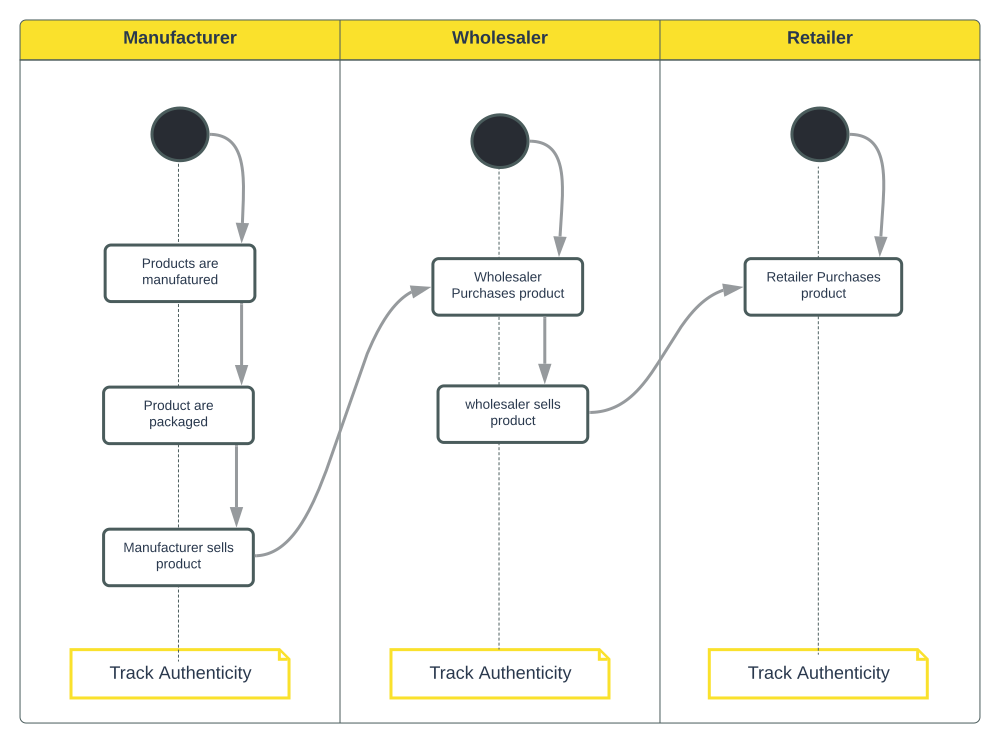
\includegraphics[width=12cm]{includes/figures/Activity Diagram.png} 
  \caption{Supply Chain Activity Diagram}
  \label{Activity Diagram}
\end{figure}

\vspace{.5cm}

The way in which files organised an classes imported using inheritance can be understand from Figure \ref{Data Model diagram}, but for the in depth understanding Figure \ref{Overall Class Diagram} should be taken into consideration.

\vspace{.5cm}
\textbf{Vyper} was also chosen to construct smart contracts, which is now one of \ac{DeFi}'s most popular languages. Vyper is a high-level programming language identical to Python. However, due to its limitations over Solidity, the proposal was subsequently abandoned.

\newpage

\begin{figure}[h]
\centering
  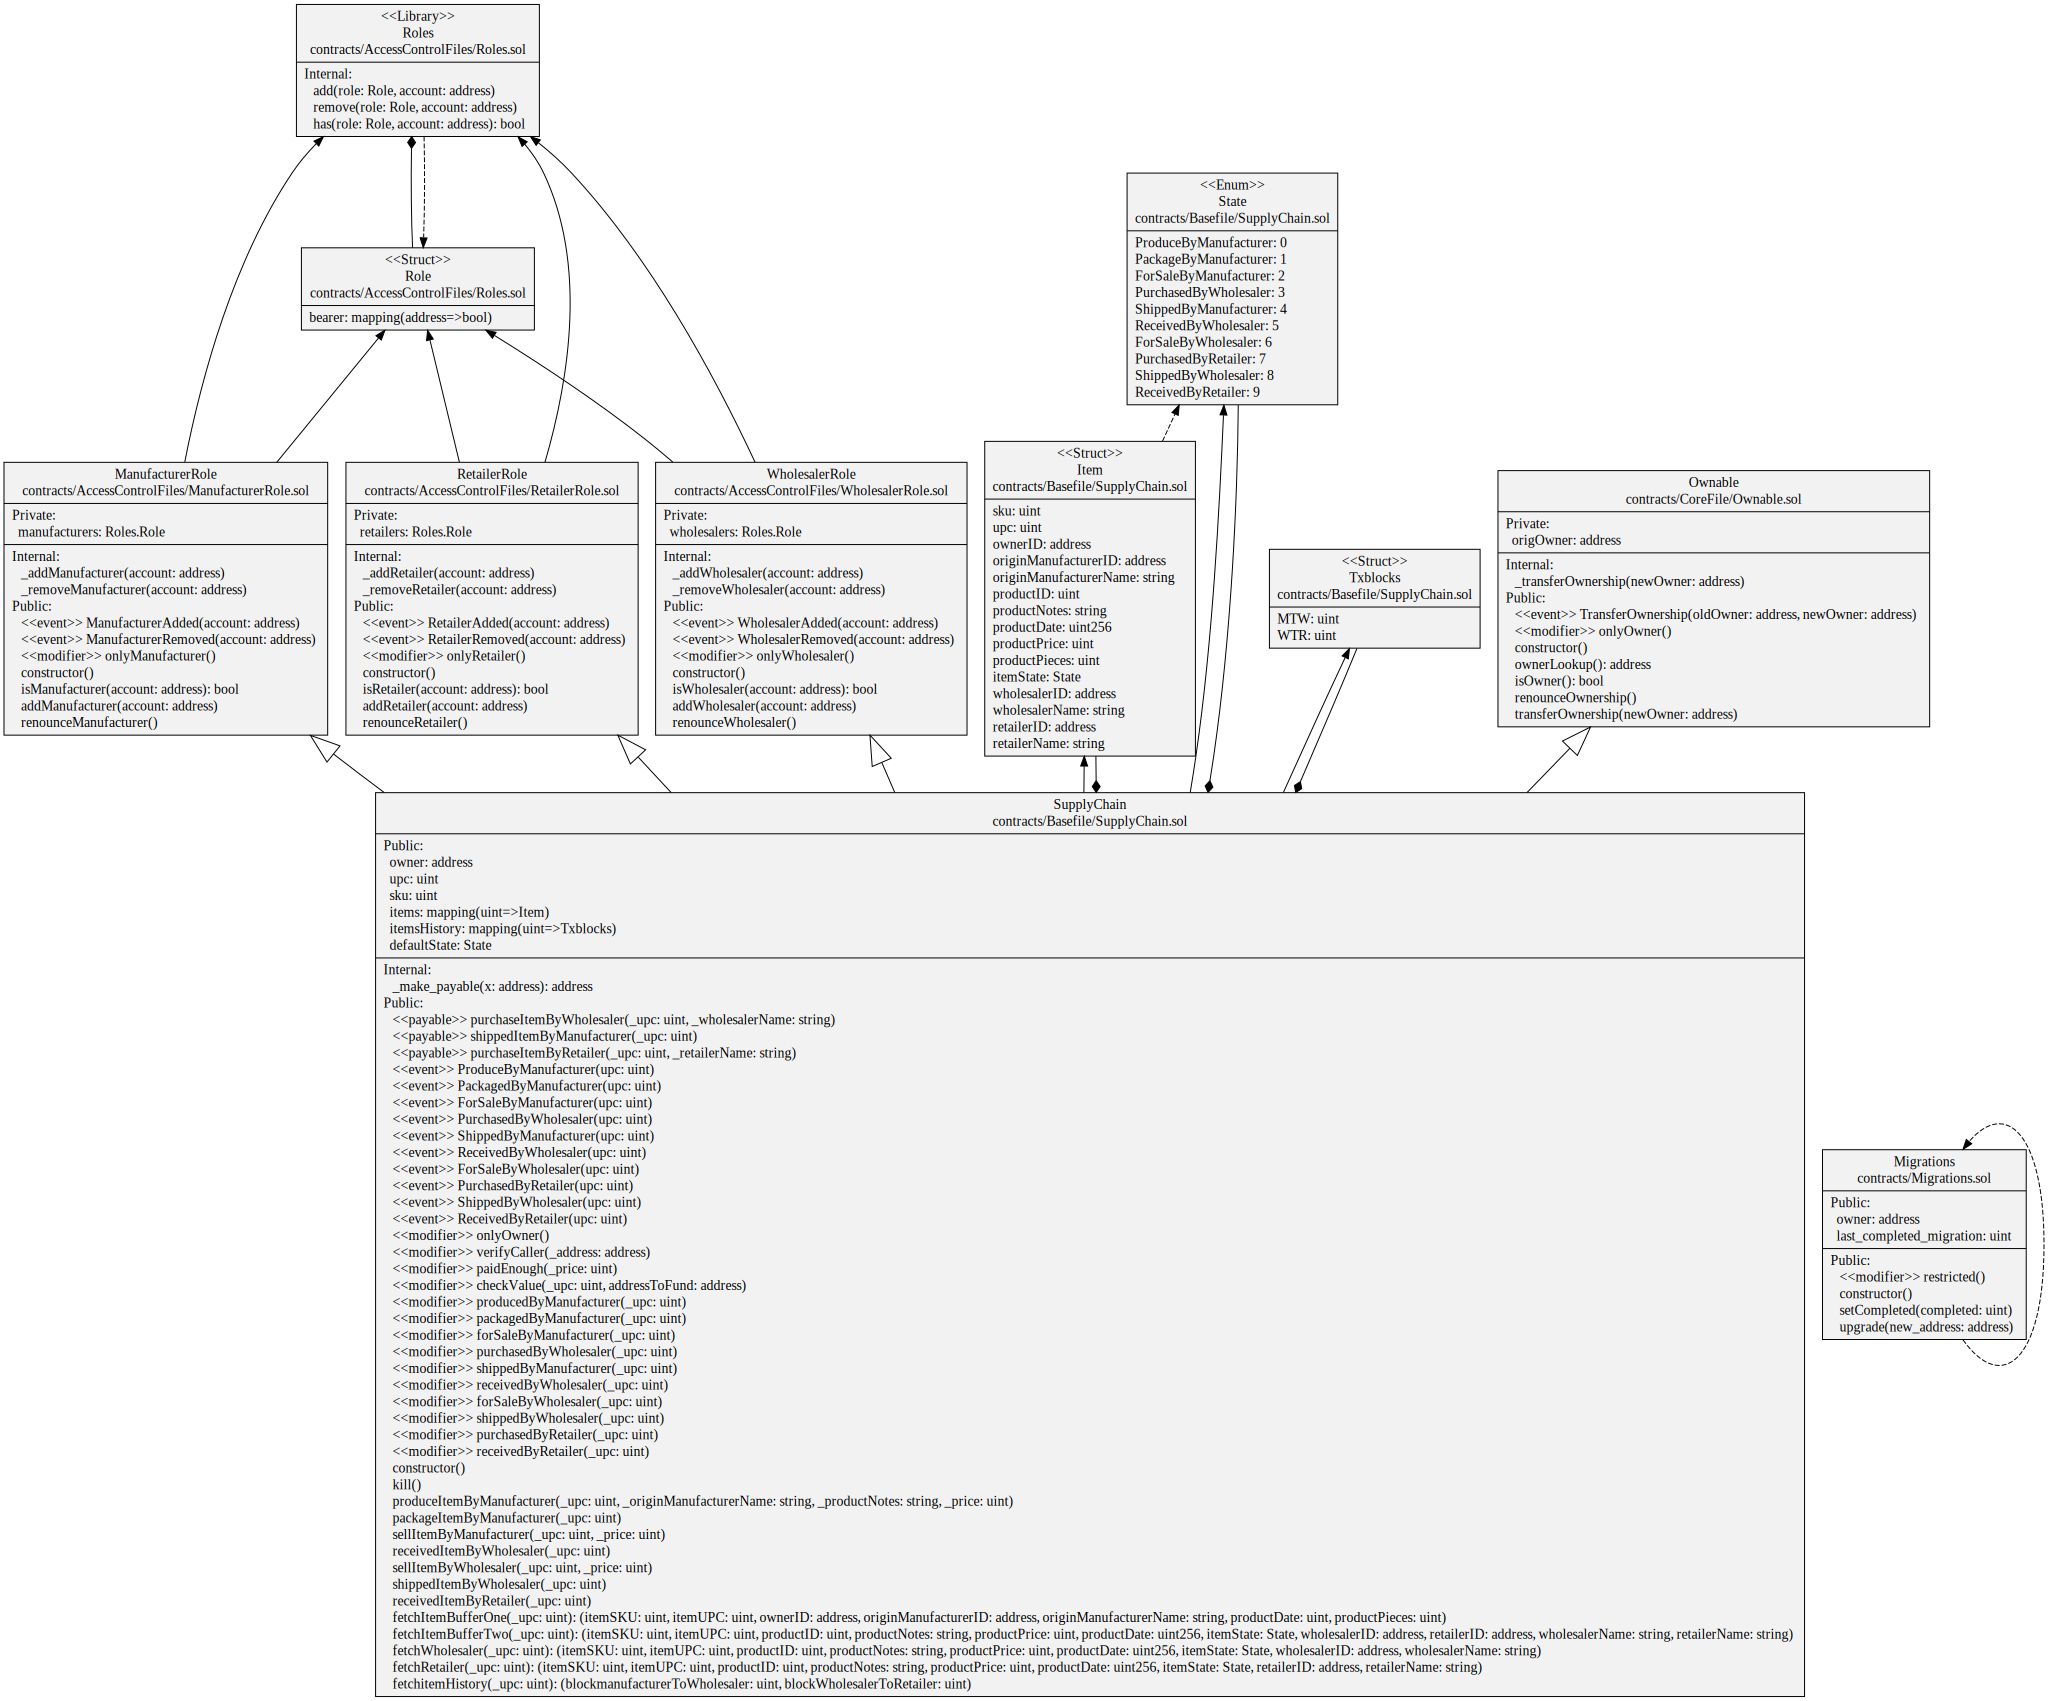
\includegraphics[width=22cm, angle=90]{includes/figures/OverallClassDiagram.png} 
  \caption{Smart Contract Class Diagram}
  \label{Overall Class Diagram}
\end{figure}

\vspace{.5cm}



\section{Integrating \ac{MAS}-\ac{BCT}}

The thesis' core premise is the integration of the two technologies, \ac{MAS} and \ac{BCT}. We have tried to integrate both the technologies using several tries by using several web3 libraries, i.e., \textit{web3.js} for JavaScript, \textit{web3.py} for Python and \textit{web3j} for Java in order to interact with Ethereum.

\subsection{Jason and Web3j}

We attempted to test each smart contract using web3js after generating them with Solidity. We considered migrating to web3j since it would be simpler as opposed to continuing to utilize Jason AgentSpeak, which is based on Java. Through the Command Line Tools tool, Web3j facilitates the development of Java smart contract function wrappers from Solidity ABI files or straight from Truffle's Contract Schema. To reveal the contract's per-network deployment address, a wrapper is "improved" and produced. When the wrapper is created, these addresses are from the truffle deployment.

\vspace{.5cm}

The plan to utilize Web3j with Jason was eventually scrapped since, in order for Jason to run \ac{MAS}, the \texttt{.mas2j} file had to be executed, and when it did, it couldn't find the \texttt{org.web3j} package. We attempted to download the jar files locally, change the version of web3j and jason, and switched from gradle to maven in order to make the program run, but the problem persisted.

\subsection{\ac{ASTRA} and Web3j}

After several attempts with web3j and Jason, we considered switching to \ac{ASTRA}, a programming language that is quite similar to Java and aims to be familiar to developers with language. A successful agent construction was followed by the same problem as with Jason when importing the web3j package.

\subsection{Jason and Web3.py}

Web3.py is a Python package that allows you to connect with Ethereum. It is often used in \ac{Dapp}s to support a number of use cases, including sending transactions, communicating with smart contracts, accessing block data, and more. The Web3.js JavaScript \ac{API} served as the foundation for the original \ac{API}, which has since expanded to meet the demands and conveniences of Python developers.

\vspace{.5cm}

Jason's Python interpreter and Web3.py worked well together. In order to communicate or convey messages from one agent to another, \texttt{.asl} files for agents were produced in Python using AgentSpeak, which is a bit different from Jason constructed using Java. Additionally, running a \texttt{.mas2j} file is not necessary for \ac{MAS} in Jason-style AgentSpeak for Python.

\subsection{Jason and Jython}

Jason AgentSpeak's smart contract development for Python and Web3py was a success. So we decided to give it another shot and try to develop it using Jython. The Jython project provides Python implementations in Java, giving Python the benefits of operating on the JVM and access to Java classes.

\vspace{.5cm}

We attempted to use Jason with Java by converting the Python code into a Java application. The creation of a Java application containing Python code was successful, but when the \texttt{.mas2j} file was executed, it was unable to import the package \texttt{org.python} , which is necessary to start the program.